\subsection{Installation einer nativen App}

\subsection{Apple iOS}

iOS ist ein Betriebssystem, welches vom US-amerikanischen Technologiekonzern \textit{Apple, Inc.} im Rahmen des erstmalig vorgestellten \textit{iPhones} im Jahre 2007, damals noch unter dem Namen \textit{iPhone OS}, in Umlauf gebracht wurde. Stand heute läuft dieses Betriebssystem ausschließlich auf den Mobilgeräte des genannten Herstellers. Neben dem iPhone nutzt auch das Multimedia-Gerät \textit{iPod touch} das Betriebssystem iOS. Der Tabletcomputer \textit{iPad} wurde bis September 2019 ebenfalls über iOS betrieben, besitzt jedoch seit der Umstellung ein eigenes, an iOS stark angelehntes Betriebssystem \textit{iPadOS}.

\subsubsection{Entwicklung von iOS-Applikationen}

In seiner ersten Version stellte iPhone OS noch keinerlei Möglichkeit bereit, Anwendungen von Drittanbietern bereitzustellen sowie zu nutzen. Dies änderte sich bei der Umbenennung des Betriebssystems in iOS im Jahre 2008, welche auch ein Software-Update zur Folge hatte, in welchem diese Eigenschaft nun geboten wurde.

\paragraph{Programmiersprache: Apple \textit{Swift}}\mbox{}\\
In der Anfangszeit der Anwendungsentwicklung für iOS wurde die bereits für andere Zwecke entwickelte und vorhandene Programmiersprache \textit{Objective-C} als Standard gewählt. Dies änderte sich im Jahre 2014, als Apple bei seiner jährlichen Entwicklerkonferenz die hauseigene Programmiersprache \textit{Swift} vorstellte, welche Objective-C in der ganzheitlichen Anwendungsenwicklung rund um Apple-Geräte ablösen sollte. In der Anfangszeit von Swift war diese immer noch stark an den Vorgänger Objective-C angelehnt. Über die Zeit sank der Einfluss, jedoch ist Swift weiterhin abwärtskompatibel zu Objective-C, welche wiederum abwärtskompatibel zu C ist.

Bei Swift handelt es sich um eine objekt- und protokoll-orientierte Programmiersprache, welche in Ihren verschiedenen Anwendungsbereichen ihre Zugehörigkeit zu verschiedenen Programmierparadigmen aufweist. Diese stützt sich vor allem auf ihrer Behauptung, möglichst leicht verständlich für einen Menschen zu sein und vermeidet bekannte Probleme anderer, populärer objektorientierter Programmiersprachen, bspw. Dereferenzierung von \texttt{null}\textit{-Pointer-Exceptions}.

Neben der Entwicklung für alle Apple-Plattformen wird Swift unter anderem auch zur Back-End-Entwicklung genutzt. Laut einer Umfrage von \textit{StackOverflow} positioniert sich Swift auf Platz 14 der beliebtesten Programmiersprachen, basierend auf 8,1\% aller Stimmen.

\paragraph{Entwicklungsumgebung: Apple \textit{Xcode}}\mbox{}\\
\textit{Xcode} ist eine, ebenfalls von Apple entwickelte, sog. integrierte Entwicklungsumgebung (engl. \ac{ide}) und wird primär für die Entwicklung von Anwendungen mit der Programmiersprache Swift eingesetzt. Grundsätzlich ist Xcode, und somit auch die Programmierung mit Swift, Apple \textit{Mac}-Nutzern vorbehalten. Über die Zeit wurden weitere \acp{ide} entwickelt, welche Swift unterstützen, denen jedoch grundlegende, nachfolgend beschriebene Funktionalitäten von Xcode, fehlen. Zu nennen ist hier bspw. die Lösung \textit{AppCode} des Unternehmens \textit{JetBrains}.

Xcode unterstützt neben Swift auch die abwärtskompatiblen Programmiersprachen Objective-C, C, aber auch C++, Python, Ruby, sowie andere. Darüber hinaus bietet Xcode einen sog. \textit{Interface Builder}, mit welchem das Front End über separate Ansichten (sog. \textit{Views}) vorbereitet werden kann. Dabei werden verschiedenste Komponenten bereitgestellt, welche via \textit{Drag'n'Drop} innerhalb der Ansichten platziert und optisch konfiguriert werden können. Auch Beziehungen zwischen den einzelnen Views können bereits hier angelegt werden. Ein Beispiel für die Nutzung des Interface Builders kann dem unten stehenden Screenshot entnommen werden.

\begin{figure}[h!]
	\centering
	\caption{Nutzung des Interface Builders in Xcode}
\end{figure}

% Erklärung des Screenshots
Die zusammengesetzten Komponenten können, ebenfalls über Drag'n'Drop in den Quellcode referenziert werden, um die Verhaltensweisen dieser programmatisch festzulegen. Ist die App in einem testreifen Zustand, kann diese direkt über Xcode emuliert werden. Es öffnet sich ein sog. \textit{Simulator}, welcher das Zielgerät mit der geöffneten Anwendung darstellt. Das Verhalten und etwaige, daraus resultierende Probleme, können somit erkannt werden, ohne, dass es ein tatsächliches, physikalisches Zielgerät bedarf. Eigenschaften, welche auf die Hardware-Komponenten des Geräts zugreifen (bspw. die eingebauten Kameras, den Bluetooth-Sensor, etc.) können mit Ausnahme des Netzwerkkarte nicht simuliert werden.

\paragraph{Softwaredesign-Muster \textit{Model-View-Controller}}\mbox{}\\ 
Apple empfiehlt als grundlegendes Prinzip für die App-Entwicklung mit Swift das Muster \textit{\ac{mvc}}, welches im Folgenden aufgeschlüsselt wird.

\begin{description}
	\item[Model] (dt. \textit{Modell} bezieht sich auf das Datenmodell und die datenbedingte Kommunikation innerhalb der Anwendung. Innerhalb von der iOS-Anwendungsentwicklung finden sich hier Quellcode-Abschnitte für die Kommunikation der App mit einer potentiellen \acs{api}, Code für die Definition und Bereitstellung von persistentem Speicher sowie die Handhabung der dadurch entstehenden Daten. Auch im Quellcode verwendete Konstanten sind dem Modell zuzuschreiben.
	\item[View] (dt. \textit{Präsentation}) bezieht sich auf die Front-End-Komponenten der Anwendung. Alle durch den Interface Builder spezifizierten Eigenschaften sind der Präsentation zuzuschreiben, also jegliche Komponenten, front-end-basierte Klassen sowie Animationen.
	\item[Controller] (dt. \textit{Steuerung}) beinhaltet die spezifische Verhaltenslogik der Anwendung bei Interaktion mit dieser durch den*die Nutzer*in. Vereinfacht formuliert bestimmt dieser, welche Funktionalität zu welcher Zeit auf Basis welches Verhaltens ausgeführt wird. Diese ist ebenfalls für die Kommunikation zwischen dem Modell und der Präsentation zuständig.
\end{description}

Die Kooperation der einzelnen Komponenten dieses Musters lässt sich anhand der unten stehenden Abbildung erläutern.

\begin{figure}[h!]
	\centering
	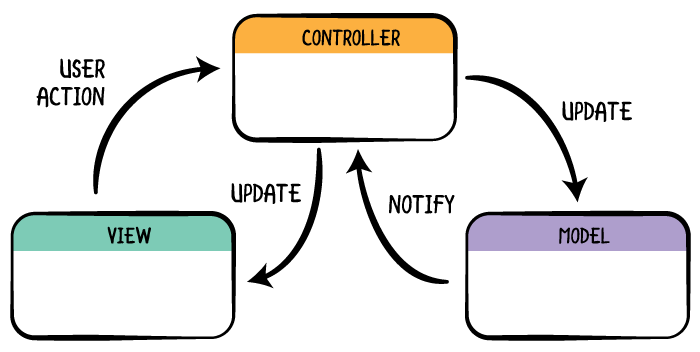
\includegraphics[width=0.5\linewidth]{img/mvc}
	\caption{Zusammenspiel des \ac{mvc}-Musters}
\end{figure}

% Erklärung MVC-Grafik

Technisch wird dieses Muster durch die Verknüpfung der einzelnen (durch den Interface Builder bereitgestellten oder erstellten) Views mit spezifischen, sog. \textit{View Controllern} realisiert. Durch eine Aktion des*der Nutzers*in auf dem View wird die entsprechende Funktionalität über den View Controller bereitgestellt. Dieser kann dan ebenfalls Funktionen ausführen, welche durch das Modell bereitgestellt werden, falls die Aktion dies bedarf. Die entsprechenden Klassen der View Controller sind Unterklassen der einzelnen, spezifischen Views, welche deren vorgesetzte Basisfunktionalitäten um die gewünschten Funktionen des*der Entwicklers*in erweitern.

\paragraph{Vorbereitung der Projektumgebung}\mbox{}\\
Bei der Erstellung eines neuen Projektes innerhalb von Xcode wählt der*die Entwickler*in bereits zu Beginn bestimmte Spezifikationen für die zu entwickelnde Anwendung. Da Swift auch für andere Betriebssysteme von Apple zur Anwendungsentwicklung genutzt wird, gehört die Spezifizierung des Anwendungsbereiches (hier: iOS) sowie des grundlegenden Aufbaus der App zu den Vorbereitungsmaßnahmen der Projektumgebung. Dieses Dialogfenster kann aus dem unten stehenden Screenshot entnommen werden.

\begin{figure}
	\centering
	\caption{Dialogfenster zum Anlegen eines neuen Projektes (Xcode)}
\end{figure}

Letztere bereiten verschiedene Dateitypen innerhalb der Umgebung vor, bspw. verschiedene Ansichten mit bereits integrierter Navigation, welche bei einer Anwendung mit nur einer Ansicht nicht zu tragen kommen. Im zweiten Schritt der Projektvorbereitung trifft der*die Entwickler*in Entscheidungen über Projektverzeichnis, -namen und -sprache sowie über weitere Projektkomponenten, welche für die Anwendung von Bedarf wären.

Alle hier getroffen Schritte können auch manuell bzw. im Nachgang der Projekterstellung angelegt werden. Grundsätzlich sind die Dateien und Quellcodezeilen, welche durch die genannten Vorbereitungsmaßnahmen automatisch generiert werden, unabdingbar für die Realisierung des Projekt und können somit für eine effizientere Arbeit des*der Entwicklers*in sorgen.

\paragraph{Struktur des initialen Entwicklungsverzeichnisses}
Bereits zu Anfang befinden sich bestimmte Dateien im Entwicklungsverzeichnis, welche sich grundsätzlich in jeder iOS-Anwendung benötigt werden. Diese werden im Folgenden beschrieben.

\begin{description}
	\item[\texttt{AppDelegate.swift}] ist der Eintrittspunkt der App. Dieser ist zuständig für das Verhalten der App, wenn diese (zum ersten Mal) geöffnet, geschlossen oder in den Hintergrund gerückt (d.\ h. inaktiv gesetzt) wird. Diese Datei ist vor allem dann von Interesse, wenn die Anwendung auch außerhalb ihrer Aktivität bestimmte Funktionen ausführt, bspw. also bei Musik-Anwendungen oder Stoppuhren. Aufgrund der automatischen Bereitstellung von Core Data zu Anfang des Projektes ist hier auch das Grundgerüst des \textit{Persistent Service} zu finden.
	\item[\texttt{SceneDelegate.swift}] ähnelt dem \texttt{AppDelegate} sehr, bezieht sich jedoch auf das Verhalten der Ansicht(-en) der Anwendung. Diese wird benötigt, da seit iOS-Version 13 auch mehrere offene Instanzen derselben App möglich sind, welche jedoch immer den aktuellsten Zustand darstellen sollen, unabhängig von der gerade aktiv laufenden Instanz. In Form einer Analogie aus der Web-Entwicklung kann man den \texttt{SceneDelegate} als die oberste Hierarchie der \textit{Front End}-Steuerung bezeichnen, während das \textit{Back End} über den \texttt{AppDelegate} orchestriert wird.
	\item[\texttt{ViewController.swift}] ist einer von beliebig vielen möglichen Controllern, welche direkte Anbindung zu einer oder mehreren Ansichten hat. Dieser beinhaltet Konfigurationen der verschiedenen Komponenten der Ansicht und spezifiziert auch das Verhalten der Ansicht, wenn auf diese oder von dieser gewechselt wird.
	\item[\texttt{Main.storyboard}] ist das Gegenstück zu den \texttt{ViewController}. In Form eines sog. \textit{Interface Builders} können verschiedene Ansichten und deren Verknüpfungen via \textit{Drag'n'Drop} erstellt werden. Jede Ansicht wird mit genau einem \texttt{ViewController} versehen, welcher die Steuerung der definierten Elemente übernimmt. Grundsätzlich ist es auch möglich, vollständig ohne Interface Builder auszukommen. Die initiale Konfiguration der Positionen und der weiteren optischen Eigenschaften wird dann ebenfalls über den entsprechenden \texttt{ViewController} gehandhabt, wobei dies einen deutlich höheren Programmieraufwand aufweisen könnte. Neben des \texttt{Main.storyboard} existiert auch ein \texttt{LaunchScreen.storyboard}, welcher beim Laden der Anwendung ausgeführt wird.
	\item[\texttt{Assets.xcassets}] beinhaltet das App-Logo, welches im Menü des Mobilgerätes angezeigt wird. Dieses muss in fest definierten Größen bereitgestellt werden, wird jedoch an dieser Stelle vernachlässigt. Darüberhinaus können hier auch alle weiteren Grafiken, etc., abgelegt werden, welche innerhalb der App genutzt werden, um für eine ordnungsgemäße Skalierung der Symbole je nach Bildschirmgröße des Endgeräts zu gewährleisten.
	\item[\texttt{Info.plist}] ist eine allgemeine Konfigurationsdatei. Diese wird u.a. für Berechtigungen genutzt, welche die Anwendung außerhalb ihres eigenen Handlungsspielraums haben soll, bspw. die Nutzung der eingebauten Kameras, des GPS-Standortes des Geräts, die Berechtigung, Benachrichtigungen anzuzeigen, etc.
	\item[\texttt{to\_do.xcdatamodeld}] stellt die Konfigurationsdatei des Persistent Service dar, sofern dieser im Dialogfenster aktiviert wurde. In dieser werden Entitäten angelegt, mit möglichen Relationen versehen und für die Verwendung innerhalb der App exportiert.
\end{description}

\subsubsection{Vertrieb von iOS-Appliaktionen}
Der mit iOS 2.0 (Nachfolger von iPhone OS) ins Leben gerufene Apple \textit{App Store} ist die einzige offizielle Bezugsstelle für iOS-Applikationen. Somit ist es auch der am meisten verwendete Marktplatz, in welchem Entwickler und Unternehmen ihre Anwendung kostenlos sowie kostenpflichtig zum Download anbieten.

Zunächst ist die Anmeldung des*der Entwicklers*in als \textit{Apple Developer} im Vorhinein von Nöten. Ohne diese könnte die Anwendung zwar programmiert und innerhalb der Entwicklungsumgebung getestet, jedoch nicht auf tatsächlichen iOS-Geräten getestet und zum Download freigegeben werden. Dies hat sowohl sicherheitstechnische als auch wirtschaftliche Gründe, welche hier nicht weiter diskutiert, jedoch für die Evaluation der Entwicklungsfreiheit in Betracht gezogen werden. Letzteres erkennt man vor allem an der Tatsache, dass die Verbreitung von Anwendungen über den \textit{App Store} kostenpflichtig ist.

% Evtl. Quelle für die App-Publikation (iOS) finden und zitieren
Der genaue Prozess der Publikation von iOS-Applikationen kann im Rahmen dieser Arbeit nicht nachvollzogen werden, da keine Möglichkeit der tatsächlichen Bereitstellung der zu entwickelnden Beispielanwendung vorliegt.

\subsubsection{Nutzung von iOS-Applikationen}
Wie im vorigen Abschnitt erwähnt werden iOS-Anwendungen im Regelfall über den App Store bezogen. Auf weitere, inoffizielle und teils nonkonforme Praktiken wie das sog. \textit{Jailbraking} des Gerätes, um auch nicht-authorisierte Anwendungen herunterladen und nutzen zu können, wird hier nicht eingegangen.

Der*die iOS-Nutzer*in sucht über den App Store die gewünschte App und lädt diese herunter. Für diesen Prozess ist eine sog. \textit{Apple ID}, also ein Benutzerkonto bei Apple von Nöten. Sollte die gewünschte App kostenpflichtig sein, so müssen Kreditkarten- oder anderweitige, valide Zahlungsdaten dem Konto hinterlegt sein. Der*die Nutzer*in bestätigt den Kauf bzw. erstmaligen Download über das Benutzerkontenpasswort oder eine gerätespezifische Authentifizierungsmethode (bspw. Fingerabdruck-Erkennung via \textit{Touch ID} oder Gesichtserkennung via \textit{Face ID}, sofern vorhanden). Daraufhin startet der Download. Die App kann über ihr korrespondierendes App-Symbol, welches nun auf dem Menü-Bildschirm des Geräts erscheint, geöffnet werden.

Falls die App in einer nun aktuelleren Version vorliegt, wird diese entweder über den App Store automatisch im Hintergrund neu heruntergeladen. Andernfalls kann der*die Nutzerin diesen Schritt auch manuell über den App Store in Kraft setzen.
